\documentclass{article}
\usepackage{tikz}
\usetikzlibrary{arrows.meta,positioning}
\usepackage[paperwidth=16.5cm,paperheight=7.4cm,margin=2mm]{geometry}
\pagestyle{empty}
\begin{document}
\centering\vspace*{\fill}
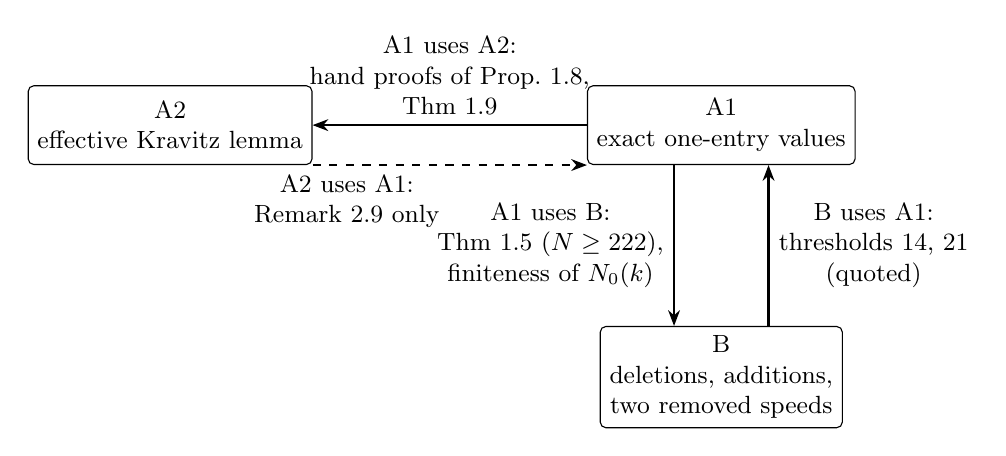
\begin{tikzpicture}[font=\small,
  paper/.style={draw,rounded corners=2pt,minimum width=3cm,minimum height=1cm,align=center},
  uses/.style={-{Stealth[length=2mm]},thick},
  weak/.style={-{Stealth[length=2mm]},thick,dashed}]
\node[paper] (A2) at (0,0) {A2\\effective Kravitz lemma};
\node[paper] (A1) at (7,0) {A1\\exact one-entry values};
\node[paper] (B)  at (7,-3.2) {B\\deletions, additions,\\two removed speeds};
\draw[uses] (A1.west) -- node[above,align=center]{A1 uses A2:\\hand proofs of Prop.~1.8,\\Thm~1.9} (A2.east);
\draw[weak] (A2.south east) -- node[below left,align=center]{A2 uses A1:\\Remark~2.9 only} (A1.south west);
\draw[uses] ([xshift=-0.6cm]A1.south) -- node[left,align=center]{A1 uses B:\\Thm~1.5 ($N\ge222$),\\finiteness of $N_0(k)$} ([xshift=-0.6cm]B.north);
\draw[uses] ([xshift=0.6cm]B.north) -- node[right,align=center]{B uses A1:\\thresholds 14, 21\\(quoted)} ([xshift=0.6cm]A1.south);
\end{tikzpicture}
\vspace*{\fill}
\end{document}
